\documentclass[letterpaper, 12pt, oneside]{article}%´
\usepackage{amsmath}%paquete para escribir expresiones matemámaticas
\usepackage{graphicx}%paquete para poder incluír imagenes en el documento
\usepackage{xcolor} %paquete de LaTex para poder poner otro texto
\graphicspath{{Imagenes/}}%directorio de la imagen, este lo cambian por el directorio en el que ustedes guardaron su imagen 1.png
\usepackage[utf8]{inputenc} %para poder poner acentos
\usepackage{listings}

\title{\Huge Taller de Herramientas Computacionales}
%\title{\Huge \colorbox{magenta}{Taller de Herramientas computacionales}} %De esta forma con colorbox pone el texto dentro de una "caja" de color.
\author{Josué Artemio Hernández Rodríguez}%autor del escrito
\date{16/01/19}%fecha del escrito

\begin{document}%inicia el documento
	\maketitle
	%\vfill %Para rellenar el espacio y colocar hasta abajo de la pagina el siguiente texto, imagen.
	\begin{center}%inicia centrado
		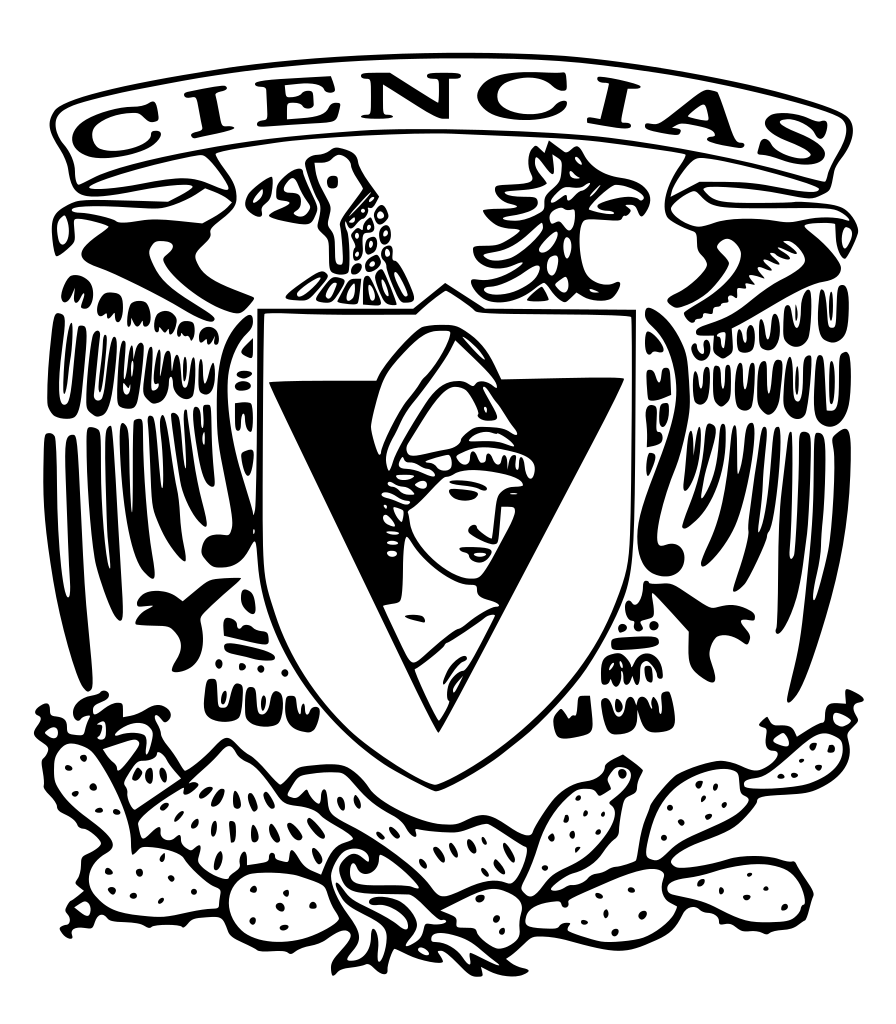
\includegraphics[scale=0.2]{2.png}%del lado izquierdo se muestra el tamaño de la imagen, del derecho se escribe el nombre de la imagen a incluir en el texto
	\end{center}%termina el centrado para la imagen
	\newpage%crea una nueva página
	
	\title{\Huge Funciones en python \\}%titulo2 
	%\\ sirven para saltar una linea.
	
	Lo que vimos en clase fue:
	\begin{enumerate}%Inicio de númeración para enlistar las cosas vistas en clase.
		\item Algunos conceptos y software utilizado en clase%item sirve enlistar el elemento, este es el primer elemento enumerado.
		\begin{itemize}
			\item Metodo: Son las acciones que realiza un objeto, modifican un objeto o hace que interaccione con otro.
			\item Dentro de una biblioteca se define una clase y en la biblioteca hay funciones o metodos (asociados a un objeto)	
			\item La diferencia de función y metodo es que una funcion no depende del objeto y el metodo si
			
		\end{itemize}
		
		\item Comandos de bash%Segundo elemento enumerado.
		\begin{itemize}%comienza el enlistado pero itemize a diferencia de enumerate enlista sin un orden secuencial (es decir no utiliza números, ni letras)
			\item ctrl + z : Pone en pausa un proceso
			\item bg : Puedo usar la terminal sin pausar los procesos
			\item "programa" \& : Arranca la aplicación "programa" pero deja libre la terminal y asi se evita tener varias ventanas de la termnal abiertas
			\item fg : Regresa a primer plano un programa despues de haberla congelado con ctrl + z
			\item kill Manda una señal a un proceso en especifico
			\item kill -9 "proceso": Cierra un proceso
			\item ls -l "archivo" :Muestra información adicional de un archivo
			\item chmod +x "archivo" : Le da atributos de ejecucion a un archivo
			\item ./ Directorio en el que estoy
			\item ../ Directorio padre
			\item where is "programa" : Busca la ruta de un programa especificado
			\item find . -name "*.py" : Busca todos los archivos con la extencion .py
		
			
		\end{itemize}%finaliza enlistado con itemize	
	\newpage
		\item Comandos y código de python
		\begin{itemize}
			\item \#!/usr/bin/python2.7  : Se coloca en nuestro programa de python para especificarle que utilice cierte interprete para ejecutarlo, en este caso es python2.7
			\item "x,y,z" Es una cadena con las variables x, y \& z
			\item x,y,z= Es una asignacion de valores
			\item 'x,y,z'. split(",") Nos separa las letras en comas
		\end{itemize}
	\item Codigo de \LaTeX
		\begin{itemize}
			\item 
				\begin{lstlisting}
\begin{bmatrix}
x_{2} & x_{3}\\
x_{4} & x_{6}\\  : Nos coloca una matriz
\end{bmatrix}
				\end{lstlisting}
			\item 
				\begin{lstlisting}
\dots : Coloca tres puntos de forma horizontal
				\end{lstlisting}
			\item 
				\begin{lstlisting}
\ddots : Coloca tres puntos de manera diagonal
				\end{lstlisting}
			\item 
				\begin{lstlisting}
\vdots : Coloca tres puntos de manera vertical
				\end{lstlisting}
			
			
			\item 
			\begin{lstlisting}
$\sum$ : Nos coloca el simbolo de suma
			\end{lstlisting}
						
		
		\end{itemize}	
		
		
		
		
	\end{enumerate}%finaliza el enlistado principal
	
	
	
\end{document}%termina el documento